
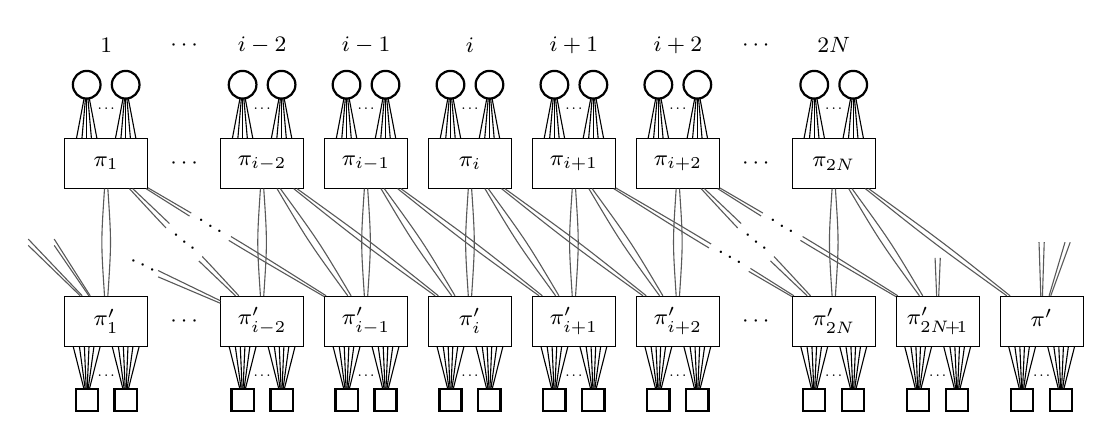
\begin{tikzpicture}[
  xscale=0.33,yscale=1,
  bitnode/.style={circle,minimum size=10pt,thick,draw=black,fill=white},
  checknode/.style={rectangle,minimum size=8pt,thick,draw=black,fill=white},
  permnode/.style={rectangle,very thin,minimum width=30pt,minimum height=18pt,fill=white,draw=black},
  permedge/.style={black!65},
  socketedge/.style={black},
  ]

  %%% Section labels
  \foreach \i/\text in {0/1,3/\cdots,6/i-2,10/i-1,14/i,18/i+1,22/i+2,25/\cdots,28/2N} {
    \node at (\i,2.5) {\footnotesize{$\text$}};
  }
  %%% 

  \def \vndist {0.75}
  \def \cndist {0.75}
  \def \vny {2}
  \def \cny {-2}

  \def \midx   {0.5}

  \foreach \x/\i/\text in {0/1/1} {
    \draw[socketedge] (\x-\vndist, \vny) +(0,0) -- +(240:1);
    \draw[socketedge] (\x-\vndist, \vny) +(0,0) -- +(255:1);
    \draw[socketedge] (\x-\vndist, \vny) +(0,0) -- +(270:1);
    \draw[socketedge] (\x-\vndist, \vny) +(0,0) -- +(285:1);
    \draw[socketedge] (\x-\vndist, \vny) +(0,0) -- +(300:1);

    \draw[socketedge] (\x-\vndist, \cny) +(0,0) -- +(52.5:1);
    \draw[socketedge] (\x-\vndist, \cny) +(0,0) -- +(67.5:1);
    \draw[socketedge] (\x-\vndist, \cny) +(0,0) -- +(82.5:1);
    \draw[socketedge] (\x-\vndist, \cny) +(0,0) -- +(97.5:1);
    \draw[socketedge] (\x-\vndist, \cny) +(0,0) -- +(112.5:1);
    \draw[socketedge] (\x-\vndist, \cny) +(0,0) -- +(127.5:1);

    \draw[socketedge] (\x+\vndist, \vny) +(0,0) -- +(240:1);
    \draw[socketedge] (\x+\vndist, \vny) +(0,0) -- +(255:1);
    \draw[socketedge] (\x+\vndist, \vny) +(0,0) -- +(270:1);
    \draw[socketedge] (\x+\vndist, \vny) +(0,0) -- +(285:1);
    \draw[socketedge] (\x+\vndist, \vny) +(0,0) -- +(300:1);

    \draw[socketedge] (\x+\vndist, \cny) +(0,0) -- +(52.5:1);
    \draw[socketedge] (\x+\vndist, \cny) +(0,0) -- +(67.5:1);
    \draw[socketedge] (\x+\vndist, \cny) +(0,0) -- +(82.5:1);
    \draw[socketedge] (\x+\vndist, \cny) +(0,0) -- +(97.5:1);
    \draw[socketedge] (\x+\vndist, \cny) +(0,0) -- +(112.5:1);
    \draw[socketedge] (\x+\vndist, \cny) +(0,0) -- +(127.5:1);

    \node[bitnode] (v1\i) at (\x-\vndist, \vny) {};
    \node[bitnode] (v2\i) at (\x+\vndist, \vny) {};
    \node[checknode] (c1\i) at (\x-\cndist, \cny) {};
    \node[checknode] (c2\i) at (\x+\cndist, \cny) {};

    \foreach \j in {-1.7,1.7} {
      \node at (\x,\j) {\tiny{$...$}};
    }

    \node[permnode] (perm1_node\i) at (\x,\vny-1) {\footnotesize{$\pi_{\text}$}};
    \node[permnode] (perm2_node\i) at (\x,\cny+1) {\footnotesize{$\pi_{\text}'$}};
  }

  \foreach \x in {3,25} {
    \foreach \y in {1,-1} {
      \node at (\x,\y) {\footnotesize{$\cdots$}};
    }
  }

  \foreach \x/\i/\text in {6/2/i-2,10/3/i-1,14/4/i,18/5/i+1,22/6/i+2,28/7/2N} {
    \draw[socketedge] (\x-\vndist, \vny) +(0,0) -- +(240:1);
    \draw[socketedge] (\x-\vndist, \vny) +(0,0) -- +(255:1);
    \draw[socketedge] (\x-\vndist, \vny) +(0,0) -- +(270:1);
    \draw[socketedge] (\x-\vndist, \vny) +(0,0) -- +(285:1);
    \draw[socketedge] (\x-\vndist, \vny) +(0,0) -- +(300:1);

    \draw[socketedge] (\x-\vndist, \cny) +(0,0) -- +(52.5:1);
    \draw[socketedge] (\x-\vndist, \cny) +(0,0) -- +(67.5:1);
    \draw[socketedge] (\x-\vndist, \cny) +(0,0) -- +(82.5:1);
    \draw[socketedge] (\x-\vndist, \cny) +(0,0) -- +(97.5:1);
    \draw[socketedge] (\x-\vndist, \cny) +(0,0) -- +(112.5:1);
    \draw[socketedge] (\x-\vndist, \cny) +(0,0) -- +(127.5:1);

    \draw[socketedge] (\x+\vndist, \vny) +(0,0) -- +(240:1);
    \draw[socketedge] (\x+\vndist, \vny) +(0,0) -- +(255:1);
    \draw[socketedge] (\x+\vndist, \vny) +(0,0) -- +(270:1);
    \draw[socketedge] (\x+\vndist, \vny) +(0,0) -- +(285:1);
    \draw[socketedge] (\x+\vndist, \vny) +(0,0) -- +(300:1);

    \draw[socketedge] (\x+\vndist, \cny) +(0,0) -- +(52.5:1);
    \draw[socketedge] (\x+\vndist, \cny) +(0,0) -- +(67.5:1);
    \draw[socketedge] (\x+\vndist, \cny) +(0,0) -- +(82.5:1);
    \draw[socketedge] (\x+\vndist, \cny) +(0,0) -- +(97.5:1);
    \draw[socketedge] (\x+\vndist, \cny) +(0,0) -- +(112.5:1);
    \draw[socketedge] (\x+\vndist, \cny) +(0,0) -- +(127.5:1);

    \node[bitnode] (v1\i) at (\x-\vndist, \vny) {};
    \node[bitnode] (v2\i) at (\x+\vndist, \vny) {};
    \node[checknode] (c1\i) at (\x-\cndist, \cny) {};
    \node[checknode] (c2\i) at (\x+\cndist, \cny) {};

    \foreach \j in {-1.7,1.7} {
      \node at (\x,\j) {\tiny{$...$}};
    }

    \node[permnode] (perm1_node\i) at (\x,\vny-1) {\footnotesize{$\pi_{\text}$}};
    \node[permnode] (perm2_node\i) at (\x,\cny+1) {\footnotesize{$\pi_{\text}'$}};
  }

  \foreach \x/\i/\text in {32/8/2N\!+\!1,36/9/\chend} {

    \draw[socketedge] (\x-\vndist, \cny) +(0,0) -- +(52.5:1);
    \draw[socketedge] (\x-\vndist, \cny) +(0,0) -- +(67.5:1);
    \draw[socketedge] (\x-\vndist, \cny) +(0,0) -- +(82.5:1);
    \draw[socketedge] (\x-\vndist, \cny) +(0,0) -- +(97.5:1);
    \draw[socketedge] (\x-\vndist, \cny) +(0,0) -- +(112.5:1);
    \draw[socketedge] (\x-\vndist, \cny) +(0,0) -- +(127.5:1);

    \draw[socketedge] (\x+\vndist, \cny) +(0,0) -- +(52.5:1);
    \draw[socketedge] (\x+\vndist, \cny) +(0,0) -- +(67.5:1);
    \draw[socketedge] (\x+\vndist, \cny) +(0,0) -- +(82.5:1);
    \draw[socketedge] (\x+\vndist, \cny) +(0,0) -- +(97.5:1);
    \draw[socketedge] (\x+\vndist, \cny) +(0,0) -- +(112.5:1);
    \draw[socketedge] (\x+\vndist, \cny) +(0,0) -- +(127.5:1);

    \node[checknode] (c1\i) at (\x-\cndist, \cny) {};
    \node[checknode] (c2\i) at (\x+\cndist, \cny) {};

    \foreach \j in {-1.7} {
      \node at (\x,\j) {\tiny{$...$}};
    }

    \node[permnode] (perm2_node\i) at (\x,\cny+1) {\footnotesize{$\pi_{\text}'$}};
  }

  %%% Sockets across permutations
  %% Straight sockets
  \foreach \x/\i in {0/1,6/2,10/3,14/4,18/5,22/6,28/7} {
%    \draw[permedge] (perm1_node\i) -- (perm2_node\i);
    \draw[permedge] (perm1_node\i) .. controls (\x-0.2,0) .. (perm2_node\i);
    \draw[permedge] (perm1_node\i) .. controls (\x+0.2,0) .. (perm2_node\i);
  }
  %% Sockets to the adjacent
  \foreach \x/\xn/\i/\j in {0/6/1/2,6/10/2/3,10/14/3/4,14/18/4/5,18/22/5/6,22/28/6/7,28/32/7/8} {
%    \draw[permedge] (perm1_node\i) -- (perm2_node\j);
    \draw[permedge] (perm1_node\i) .. controls (0.5*\x+0.5*\xn-0.2,0) .. (perm2_node\j);
    \draw[permedge] (perm1_node\i) .. controls (0.5*\x+0.5*\xn+0.2,0) .. (perm2_node\j);
  }
  \node[fill=white,rotate=-38] at (3,0) {\footnotesize{$\cdots$}};
  \node[fill=white,rotate=-38] at (25,0) {\footnotesize{$\cdots$}};

  %% Sockets to the adjacent to adjacent
  \foreach \x/\xn/\i/\j in {0/10/1/3,6/14/2/4,10/18/3/5,14/22/4/6,18/28/5/7,22/32/6/8,28/36/7/9} {
 %   \draw[permedge] (perm1_node\i) -- (perm2_node\j);
    \draw[permedge] (perm1_node\i) .. controls (0.5*\x+0.5*\xn-0.2,0) .. (perm2_node\j);
    \draw[permedge] (perm1_node\i) .. controls (0.5*\x+0.5*\xn+0.2,0) .. (perm2_node\j);
  }
  \node[fill=white,rotate=-30] at (4,0.2) {\footnotesize{$\cdots$}};
  \node[fill=white,rotate=-30] at (24,-0.2) {\footnotesize{$\cdots$}};
  \node[fill=white,rotate=-30] at (26,0.2) {\footnotesize{$\cdots$}};

  \draw[permedge] (perm2_node1) -- (-2,0.04);
%  \draw[permedge] (perm2_node1) -- (-2,0);
  \draw[permedge] (perm2_node1) -- (-2,-0.04);

  \draw[permedge] (perm2_node1) -- (-3,0.04);
%  \draw[permedge] (perm2_node1) -- (-3,0);
  \draw[permedge] (perm2_node1) -- (-3,-0.04);

  \draw[permedge] (perm2_node2) -- (2,-0.44);
%  \draw[permedge] (perm2_node2) -- (2,-0.4);
  \draw[permedge] (perm2_node2) -- (2,-0.36);
  \node[rotate=-26] at (1.4,-0.3) {\footnotesize{$\cdots$}};

  \draw[permedge] (perm2_node8) -- (32.1,-0.2);
%  \draw[permedge] (perm2_node8) -- (32,-0.2);
  \draw[permedge] (perm2_node8) -- (31.9,-0.2);

  \draw[permedge] (perm2_node9) -- (36.1,0);
%  \draw[permedge] (perm2_node9) -- (36,0);
  \draw[permedge] (perm2_node9) -- (35.9,0);

  \draw[permedge] (perm2_node9) -- (37.1,0);
%  \draw[permedge] (perm2_node9) -- (37,0);
  \draw[permedge] (perm2_node9) -- (36.9,0);

\end{tikzpicture}

%%% Local Variables: 
%%% mode: latex
%%% TeX-master: "../poster"
%%% End: 

